\section{}
A steel rod of constant flexural rigidity is described by Fig. \ref{fig:Q3ProblemDiagram}. For force P applied
at the simply supported end, derive a formula for roller reaction Q. Apply Castigliano's theorem.

\begin{figure}[h]
    \centering
    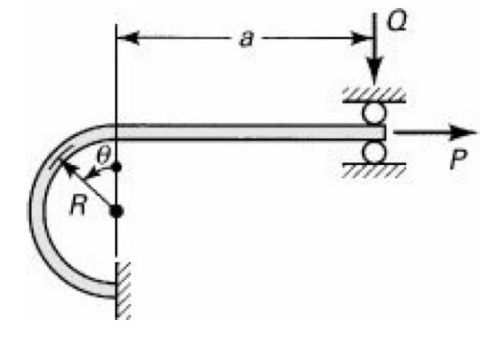
\includegraphics[width=0.3\linewidth]{Questions/Figures/Q3ProblemDiagram.png}
    \caption{Problem diagram for Question 3.}
    \label{fig:Q3ProblemDiagram}
\end{figure}

The moment equation of the straight section is:
\begin{align*}
    M &= -Q x \\
    \implies \frac{\partial M}{\partial Q} &= -x 
\end{align*}

For the curved section, a cut is made. The FBD is shown in Fig. \ref{fig:Q3FBD}.
\begin{figure}[h]
    \centering
    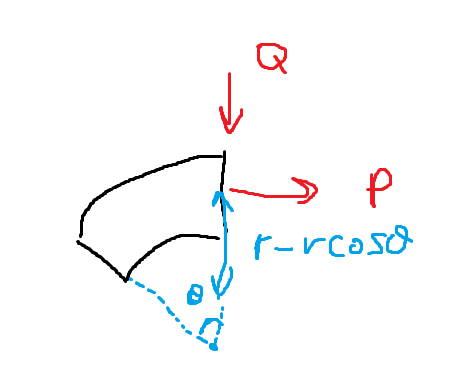
\includegraphics[width=0.4\linewidth]{Questions/Figures/Q3FBD.png}
    \caption{Free body diagram of the curved section.}
    \label{fig:Q3FBD}
\end{figure}

The equation of the moment is:
\begin{align*}
    M &= M_a - QR \sin\theta - PR(1-\cos\theta) \\
    &= -Q(a + R \sin\theta) - PR(1-\cos\theta) \\
    \implies \frac{\partial M}{\partial Q} &= -a - R \sin\theta
\end{align*}

The roller cannot carry a deflection. By Castigliano's theorem, 
\begin{align*}
    \delta_Q &= \frac{1}{EI} \left[\int_{0}^{a} M \frac{\partial M}{\partial Q} dx + 
    \int_{0}^{\pi} M \frac{\partial M}{\partial Q} R d\theta \right] \overset{\text{set}}{=} 0 \\
    \implies 0 &= \int_{0}^{a} Qx^2 dx + \int_{0}^{\pi} QR(a+R\sin\theta)^2 - PR^2(1-\cos\theta)(a+R\sin\theta) d\theta 
\end{align*}

By CAS software (Matlab Symbolic Toolbox), the integral is:
\begin{align*}
    0 &= \frac{Qa^3}{3} + 2P R^3 + \frac{Q\pi R^3}{2} + 4QR^2a + \pi PR^2a + \pi QRa^2 \\
    \implies Q &= \boxed{\frac{-PR^2(2R + a \pi)}{\frac{a^3}{3} + R(4Ra + \frac{\pi R^2}{2} + \pi a^2)}}
\end{align*}